\pagestyle{fancy}
\section{Introducción}

AironTools es una empresa mexicana con más de una década de experiencia en la producción y comercialización de herramientas industriales. A lo largo de su trayectoria ha consolidado una base de clientes recurrentes en el sector industrial mécanico y automotriz. Sin embargo, actualmente enfrenta importantes desafíos operativos derivados del uso de procesos manuales y herramientas no integradas para la gestión interna y la atención a clientes.

La gestión de servicios técnicos, inventario, comunicación interna y control de información se realiza mediante hojas de cálculo y formatos físicos, lo que ha derivado en dificultades para la trazabilidad de los servicios, errores en el registro de información, pérdida de datos importantes para la toma de decisiones, y una experiencia limitada para el cliente, al no contar con un sistema que le permita dar seguimiento a sus solicitudes de manera eficiente.

Estas deficiencias afectan directamente la eficiencia operativa, la competitividad y la capacidad de crecimiento de AironTools frente a otras empresas del sector que ya operan con sistemas digitales robustos e interconectados. En este contexto, se propone el diseño e implementación de un sistema de gestión empresarial que permita digitalizar y automatizar los procesos clave de la organización.

El objetivo del proyecto es desarrollar una plataforma integral que centralice la información, mejore la trazabilidad de los servicios ofrecidos, optimice el control de inventario y facilite la comunicación entre las distintas áreas operativas. Este sistema estará alineado con los flujos de trabajo actuales de la empresa, y se construirá bajo una arquitectura escalable que garantice su adaptabilidad y crecimiento a futuro.

Como beneficio, se espera una mejora sustancial en los tiempos de respuesta, una administración más eficiente de los recursos, una atención al cliente más ágil y profesional, y un fortalecimiento de la capacidad competitiva de AironTools en el mercado de herramientas industriales. El presente proyecto se enmarca dentro de la modalidad de experiencia profesional, y responde a una necesidad real detectada en la operación de la empresa.

\section{Justificación}

La propuesta de este proyecto surge de una necesidad concreta identificada en la operación diaria de la empresa AironTools. En la actualidad, la falta de un sistema de gestión empresarial digitalizado ha derivado en múltiples dificultades operativas, entre las que destacan una atención deficiente al cliente, escasa trazabilidad de los servicios técnicos, desorganización en el control de inventario y una gestión interna basada en registros manuales. Esta situación ha limitado significativamente la capacidad de la empresa para escalar sus operaciones y mantenerse competitiva frente a organizaciones del mismo sector que ya han implementado soluciones tecnológicas robustas.

Los registros actuales de clientes, servicios, inventario y empleados se realizan mediante formatos físicos o archivos aislados, lo cual genera errores frecuentes, pérdida de información, duplicidad de datos y demoras en la atención. Estas deficiencias impactan de manera directa en la eficiencia del personal, en la capacidad de respuesta y en la imagen profesional que la empresa proyecta a sus clientes.

Frente a este panorama, la implementación de un sistema de gestión empresarial integral representa una solución estratégica. Este sistema permitirá centralizar en una sola plataforma la información relacionada con empleados, clientes, servicios y productos, lo que facilitará la trazabilidad del flujo de trabajo desde la solicitud de un servicio hasta la entrega final. Además, la automatización de notificaciones y la digitalización de los procesos permitirán establecer una comunicación más eficiente con los clientes, otorgándoles información puntual y transparente sobre el avance de sus solicitudes.

Otra ventaja clave de esta solución es la optimización del control de inventario. A través de funciones como reportes automático, será posible reducir errores, evitar datos faltantes críticos en documentaciones técnicas y anticipar necesidades operativas. A su vez, los reportes generados por el sistema facilitarán la toma de decisiones basadas en datos reales y actualizados, incrementando la capacidad de análisis y planificación de la empresa.

En conjunto, esta propuesta tecnológica contribuirá a mejorar la productividad interna, profesionalizar la operación diaria y elevar la calidad del servicio ofrecido a los clientes. También permitirá documentar formalmente los procesos internos, asegurando su replicabilidad y continuidad. La digitalización de estas funciones no solo responde a una necesidad interna urgente, sino que posiciona a AironTools como una empresa moderna, eficiente y con visión de crecimiento sostenible en un mercado altamente competitivo.

\section{Objetivo general}
Diseñar un sistema digital de gestión empresarial para AironTools que automatice y centralice los procesos internos de atención al cliente, servicios técnicos, control de inventario y comunicación organizacional, con el fin de mejorar la eficiencia operativa, la trazabilidad de los servicios y la calidad del servicio ofrecido.

\section{Objetivos específicos}
\begin{enumerate}
	\item Desarrollar un módulo de gestión de usuarios que permita registrar, organizar y asignar roles diferenciados al personal de AironTools según sus funciones operativas mediante permisos.

	\item Implementar un módulo de gestión de clientes que facilite el registro, seguimiento del historial de atención y mejora en la comunicación con los clientes.

	\item Automatizar el flujo completo de los servicios técnicos, desde el ingreso del equipo hasta su entrega, integrando notificaciones en cada etapa del proceso.

	\item Diseñar un módulo de control de inventario que permita registrar, editar y consultar productos con sus respectivos detalles, funcionando como catálogo actualizado de herramientas.
\end{enumerate}

\section{Trabajos relacionados}

A continuación se presentan ocho trabajos que abordan problemáticas similares a las identificadas en el presente proyecto. Se analiza su propósito, contexto, solución implementada y resultados obtenidos, con el fin de establecer un marco de referencia que oriente el diseño del sistema propuesto para AironTools.

\subsection{Elaboración de un sistema de gestión por procesos aplicado a una empresa dedicada a la distribución y comercialización de productos de ferretería y materiales de construcción \cite{Vargas2018}.}

Este proyecto integrador fue desarrollado en la Escuela Superior Politécnica del Litoral, Ecuador, con el objetivo de mejorar la eficiencia operativa de una empresa ferretera mediante la estandarización de sus procesos. La organización enfrentaba problemas de control interno, duplicidad de funciones y bajo aprovechamiento de recursos. Para atender esta situación, se diseñó un sistema de gestión basado en procesos, levantando y documentando operaciones clave como recepción, almacenaje, facturación y distribución. Se aplicaron herramientas como análisis FODA, flujogramas, metodología 5W+1H, diagrama de Ishikawa e indicadores de desempeño. Como resultado, se estructuró una propuesta organizacional orientada a optimizar la toma de decisiones, fortalecer el control administrativo y elevar la competitividad en el mercado.

\subsection{Desarrollo de un sistema de gestión por procesos para empresas de servicios de ingeniería y construcción orientadas a la industria \cite{Munoz2018}.}

Esta tesis de maestría tuvo como finalidad mejorar la eficiencia organizacional de la empresa CDM S.A., dedicada a servicios industriales de ingeniería y construcción, mediante el diseño de un sistema de gestión por procesos. La empresa presentaba deficiencias en la estandarización de actividades, fallos de comunicación entre áreas y ausencia de documentación formal. La propuesta se basó en teorías administrativas contemporáneas y en la norma ISO 9001:2015, integrando procesos estratégicos, operativos y de apoyo, con herramientas como mapas de procesos, diagramas de flujo, políticas, indicadores y mecanismos de mejora continua. El resultado fue un modelo estructurado que facilita la documentación, el control y la mejora de las operaciones clave.

\subsection{Diseño de un sistema de gestión basado en procesos \cite{Jacome2016}.}

Esta tesis de maestría, desarrollada en la Universidad Andina Simón Bolívar, propuso un sistema de gestión basado en procesos para una empresa de tecnología que enfrentaba desorganización operativa y baja eficiencia administrativa. Con el fin de mejorar la rentabilidad y el control interno, se estructuró una solución fundamentada en normas ISO, análisis detallado de procesos, definición de indicadores de desempeño y documentación formal. El resultado fue un modelo que fortaleció la claridad organizacional y facilitó la toma de decisiones mediante una gestión alineada a objetivos estratégicos.

\subsection{Proceso Administrativo y Gestión Empresarial en COPROABAS, Jinotega \cite{Flores15}.}

Esta tesis de maestría tuvo como propósito mejorar el desempeño organizacional de la cooperativa COPROABAS mediante el fortalecimiento de su gestión administrativa. La investigación identificó deficiencias en la estructuración organizativa, ausencia de manuales de funciones y falta de cultura administrativa. A partir de un enfoque descriptivo y transversal, se evaluó la aplicación del proceso administrativo y se propusieron mejoras orientadas a optimizar la planificación, organización, dirección y control dentro de la cooperativa.

\subsection{Principales causas del fracaso en la implementación de un ERP: el caso de una PyME en México \cite{Delgado2015}.}

Esta tesis de maestría desarrollada en la UNAM tuvo como finalidad identificar las causas que provocan el fracaso en la implementación de sistemas ERP en pequeñas y medianas empresas mexicanas. Mediante el método Delphi aplicado a expertos, se detectaron deficiencias en la capacitación, selección de personal y planeación estratégica. El estudio evidenció una limitada cultura tecnológica y desinterés gerencial como factores críticos, y concluyó con recomendaciones orientadas a mejorar la preparación y ejecución de futuros proyectos de ERP en el entorno PyME.

\subsection{Planeación Estratégica y Nuevos Proyectos en Empresa Propia \cite{Patino19}.}

Este proyecto terminal, desarrollado en la Universidad ICESI, tuvo como objetivo consolidar la planeación estratégica de una empresa apícola en fase inicial. La propuesta abordó la falta de estructura organizacional mediante el análisis FODA, el modelo Canvas y herramientas de diagnóstico interno. Se definieron la misión, visión y objetivos estratégicos, acompañados de proyecciones financieras, con el fin de orientar su crecimiento competitivo dentro del mercado colombiano.

\subsection{La gestión empresarial como factor clave de desarrollo de las spin-offs universitarias \cite{Rodeiro2012}.}

Este artículo, publicado en *Observatorio de la Economía Latinoamericana*, estudia las causas del bajo rendimiento de las spin-offs universitarias en Galicia, España, a pesar de su origen en entornos de alta investigación. Mediante un análisis basado en encuestas aplicadas a responsables de estas empresas, se identificaron como principales obstáculos la escasa experiencia en gestión, la débil estructura organizativa y las limitaciones financieras. El trabajo concluye con la recomendación de fortalecer las capacidades administrativas desde las etapas iniciales del emprendimiento.

\subsection{Gestión Empresarial y Desarrollo \cite{Reyes12}.}

Esta tesis doctoral plantea un enfoque sistémico y estratégico de la gestión empresarial, integrando el análisis del entorno interno, las relaciones inmediatas de la organización y el contexto macroeconómico. Aunque se trata de un estudio teórico, propone modelos referenciales y recomendaciones prácticas orientadas al fortalecimiento organizacional, con énfasis en la sostenibilidad, el desarrollo humano y la adaptación a contextos complejos.

% NOTA: Actualizar también la tabla de comparación si es necesario.


\begin{longtable}{m{.05\paperwidth} *{2}{m{.33\paperwidth}} @{}}
	\caption{Comparación cualitativa de los trabajos relacionados con el proyecto.}
	\label{table:trabajosRelacionados}\\
	\hline
	\textbf{Ref.} & \textbf{Similitudes} & \textbf{Diferencias} \\
	\hline
	\endfirsthead
	
	\multicolumn{3}{c}{\textbf{Continuación de la Tabla \ref{table:trabajosRelacionados}}} \\
	\hline
	\textbf{Ref.} & \textbf{Similitudes} & \textbf{Diferencias} \\
	\hline
	\endhead
	\hline
	\endlastfoot

	\cite{Vargas2018} &
	\begin{itemize}
	  \item Ambos proyectos aplican la gestión por procesos como enfoque estructural.
	  \item Se busca mejorar la eficiencia operativa y la toma de decisiones empresariales.
	  \item Se parte de problemáticas internas como falta de control, duplicidad de funciones y baja eficiencia.
	\end{itemize} &
	\begin{itemize}
	  \item El proyecto de Vargas empleó herramientas formales como FODA y KPIs; en mi caso se realizó un diagnóstico documentado a partir de observaciones y reuniones internas, sin metodologías académicas específicas.
	  \item No se contempla desarrollo tecnológico; mi sistema incluye una plataforma funcional con backend, frontend y despliegue en la nube.
	  \item Su enfoque es contable y administrativo; el mío abarca trazabilidad digital, soporte técnico, automatización y arquitectura multitenant.
	\end{itemize} \\	
\midrule

\cite{Munoz2018} &
\begin{itemize}
  \item Ambos proyectos proponen un sistema de gestión centrado en procesos estratégicos, clave y de soporte.
  \item Las deficiencias internas detectadas sirvieron como base para diseñar la solución.
  \item En ambos casos, se busca mejorar la estructura organizacional mediante el rediseño de procesos.
\end{itemize} &
\begin{itemize}
  \item El proyecto de Muñoz no desarrolló un sistema digital; mi propuesta implementa una plataforma completa usando NestJS, React y MongoDB.
  \item Su enfoque es documental y administrativo; el mío automatiza procesos, permite trazabilidad digital y comunicación en tiempo real.
  \item Mi solución está desplegada en la nube y diseñada para escalar bajo una arquitectura modular y multitenant.
\end{itemize} \\


\cite{Jacome2016} &
\begin{itemize}
  \item Ambos proyectos están centrados en sistemas de gestión orientados a procesos.
  \item Se busca estructurar operaciones críticas con enfoque organizacional y mejorar la eficiencia interna.
  \item En ambos casos, se reconoce la necesidad de controlar y optimizar procesos empresariales clave.
\end{itemize} &
\begin{itemize}
  \item La tesis propone una solución conceptual y documental; mi proyecto desarrolla una plataforma funcional con tecnologías como NestJS, React y MongoDB.
  \item Mi sistema integra comunicación en tiempo real, automatización de tareas, y está desplegado en la nube con arquitectura escalable.
  \item Está orientado al sector industrial de herramientas y servicios técnicos, no al sector tecnológico-comercial.
\end{itemize} \\


\cite{Flores15} &
\begin{itemize}
  \item Ambos trabajos parten del análisis de fallas organizacionales y buscan fortalecer la gestión empresarial.
  \item Se enfocan en mejorar el desempeño general de la organización mediante la reestructuración de funciones clave.
  \item En ambos casos, se identifican problemas derivados de una gestión deficiente y se proponen soluciones concretas.
\end{itemize} &
\begin{itemize}
  \item La tesis emplea un enfoque cualitativo tradicional; mi proyecto desarrolla una solución digital funcional e implementada.
  \item Mi sistema utiliza tecnologías modernas como NestJS, React y MongoDB, integrando automatización y trazabilidad.
  \item Incluye comunicación en tiempo real y soporte multitenant, elementos ausentes en el trabajo de Flores.
\end{itemize} \\


\cite{Delgado2015} &
\begin{itemize}
  \item Ambos proyectos abordan problemáticas relacionadas con eficiencia organizacional y el uso de herramientas tecnológicas en empresas.
  \item Coinciden en señalar que una gestión adecuada de procesos es fundamental para lograr buenos resultados empresariales.
  \item Ambos consideran que la estructura organizacional y el rol del personal son relevantes para la efectividad de las soluciones implementadas.
\end{itemize} &
\begin{itemize}
  \item Mientras Delgado analiza causas de fracaso en ERPs, mi proyecto desarrolla una solución funcional con NestJS, React y MongoDB.
  \item Su enfoque es teórico y diagnóstico; el mío es aplicado, con un sistema en funcionamiento dentro de una empresa real.
  \item Mi solución automatiza procesos, incluye trazabilidad y comunicación digital, mientras que Delgado se enfoca en recomendaciones preventivas.
\end{itemize} \\


\cite{Patino19} &
\begin{itemize}
  \item Ambos proyectos surgen a partir de una necesidad empresarial real en organizaciones jóvenes.
  \item Tienen como propósito fortalecer la estructura interna de la empresa para mejorar su eficiencia operativa.
  \item En ambos casos, se busca consolidar procesos que apoyen el crecimiento competitivo en el mercado.
\end{itemize} &
\begin{itemize}
  \item El proyecto de Kopec se enfoca en planeación estratégica con herramientas como FODA y Canvas; en mi caso, la estructuración fue funcional, basada en necesidades detectadas internamente.
  \item Kopec no implementa soluciones tecnológicas; AironTools incluye un sistema completo con backend, frontend y base de datos en la nube.
  \item Mi sistema incorpora automatización, comunicación en tiempo real, soporte multitenant e infraestructura DevOps, elementos no abordados en el trabajo de Patiño.
\end{itemize} \\


\cite{Rodeiro2012} &
\begin{itemize}
  \item Ambos trabajos reconocen la importancia de la gestión empresarial como clave para la sostenibilidad y crecimiento organizacional.
  \item Se abordan barreras estructurales y organizativas que deben atenderse para mejorar el desempeño de una empresa.
  \item Se destaca la necesidad de fortalecer procesos de gestión desde etapas tempranas del desarrollo empresarial.
\end{itemize} &
\begin{itemize}
  \item El artículo se centra en el análisis de spin-offs universitarias mediante encuestas y datos estadísticos, mientras que en mi proyecto se desarrolla e implementa una solución tecnológica real en una empresa del sector industrial.
  \item En el trabajo analizado se identifican debilidades en capacidades administrativas, mientras que en mi proyecto se crean herramientas específicas para solucionar dichas deficiencias, como módulos de control, automatización, reportes y trazabilidad.
  \item El artículo propone recomendaciones generales sobre gestión y financiación; en cambio, mi propuesta incluye la integración de tecnologías como NestJS, React, MongoDB y despliegue en AWS.
\end{itemize} \\

\cite{Reyes12} &
\begin{itemize}
  \item Ambos trabajos abordan la gestión empresarial como medio para mejorar el desempeño organizacional.
  \item Se reconoce la relevancia de analizar factores internos para proponer soluciones estructurales efectivas.
  \item En ambos casos, se propone una reorganización basada en principios de eficiencia y mejora continua.
\end{itemize} &
\begin{itemize}
  \item El proyecto de Reyes es conceptual y teórico, mientras que el mío es aplicado y funcional dentro de una empresa real.
  \item Reyes no desarrolla software; mi sistema fue implementado con tecnologías como NestJS, React, MongoDB y desplegado en la nube.
  \item Su enfoque está orientado al desarrollo humano y sostenibilidad; el mío prioriza la eficiencia operativa, automatización y trazabilidad digital.
\end{itemize} \\
\bottomrule
\end{longtable}

	

\section{Descripción técnica}

El sistema propuesto para AironTools es una aplicación web de gestión empresarial compuesta por módulos funcionales independientes que automatizan y centralizan los procesos clave de la organización. Está orientado a mejorar la atención al cliente, la administración de servicios técnicos, el control de productos y la coordinación interna. Todos los módulos interactúan bajo una arquitectura escalable y mantenible, permitiendo su crecimiento progresivo.

\subsection*{Arquitectura general del sistema}

El sistema sigue una arquitectura modular cliente-servidor, donde el backend y el frontend se desarrollan de forma desacoplada. La comunicación entre ambos se realiza mediante APIs RESTful. Esta estructura permite una mayor flexibilidad, mantenibilidad y facilidad de integración futura con nuevas funcionalidades.

La Figura~\ref{fig:arquitectura} muestra una vista general de la arquitectura del sistema con sus principales componentes.

\begin{figure}[H]
	\centering
	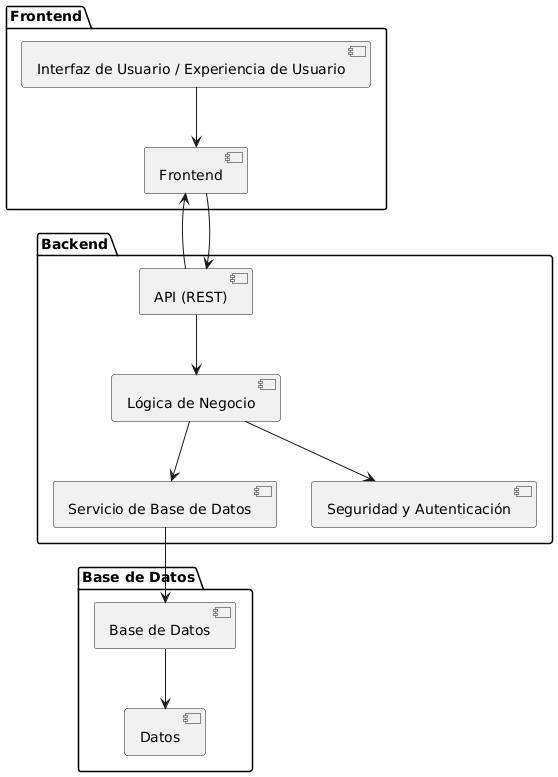
\includegraphics[width=0.6\textwidth]{sistema.png}
	\caption{Arquitectura general del sistema propuesto para AironTools.}
	\label{fig:arquitectura}
\end{figure}

\subsection*{Módulo de usuarios y roles}

Este módulo permite registrar empleados, asignar roles diferenciados y gestionar permisos de acceso al sistema. Incluye funcionalidades de autenticación y autorización para garantizar la seguridad del sistema, además de una interfaz de administración para el rol de superadministrador.

\subsection*{Módulo de clientes}

Permite registrar tanto a clientes individuales como a empresas, asociando datos de contacto e historial de servicios recibidos. Este módulo se integra con el sistema de notificaciones para mantener informados a los clientes durante cada etapa del servicio técnico.

\subsection*{Módulo de servicios técnicos}

Automatiza el flujo completo de atención a servicios como reparación, mantenimiento, demostración y cotización. El sistema registra desde el ingreso del equipo hasta su diagnóstico, reparación, validación final y entrega al cliente. Se incluyen notificaciones automáticas por cambios de estado.

\begin{figure}[H]
	\centering
	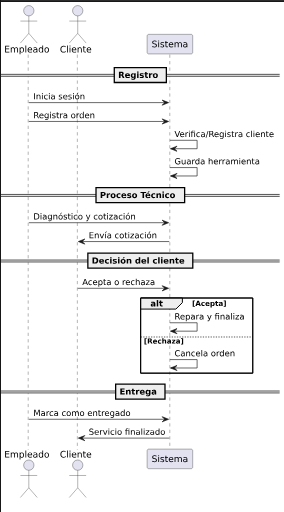
\includegraphics[width=0.4\textwidth]{secuencia-sistema.png}
	\caption{Diagrama de secuencia del flujo de atención a servicios técnicos.}
	\label{fig:secuencia}
\end{figure}

\begin{figure}[H]
	\centering
	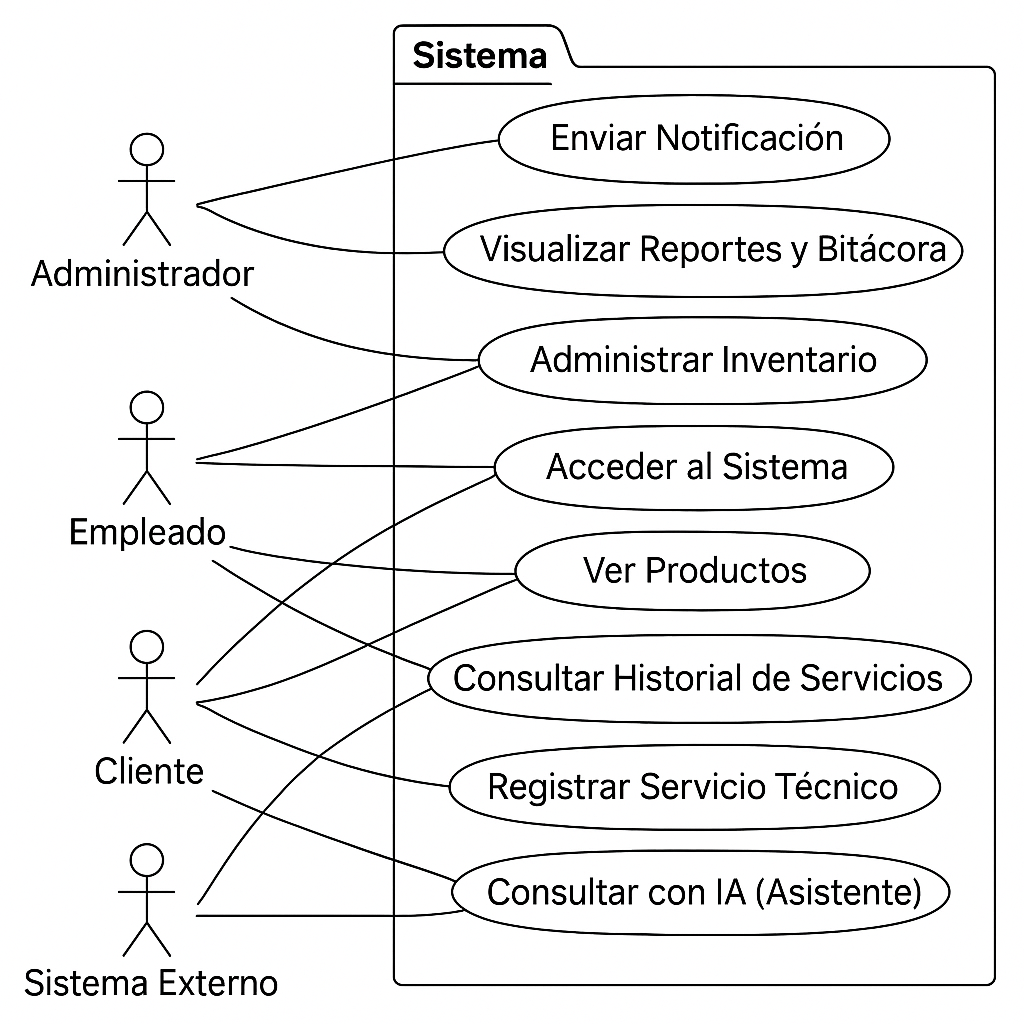
\includegraphics[width=0.6\textwidth]{casos-uso-sistema.png}
	\caption{Diagrama de casos de uso asociados a los módulos funcionales del sistema.}
	\label{fig:casosuso}
\end{figure}

\subsection*{Módulo de productos}

Este módulo permite registrar, editar y consultar productos e insumos disponibles para la venta o uso interno. Los productos se organizan jerárquicamente en familias, categorías y subcategorías, con información como nombre, precio, descripción, imágenes y diagramas técnicos. Actualmente funciona como un catálogo visual centralizado, integrable con los servicios y clientes.

\subsection*{Módulo de notificaciones y comunicación interna}

El sistema integra notificaciones por correo electrónico según el estado del servicio. También se contempla un sistema básico de comunicación en tiempo real mediante WebSockets para uso interno entre áreas operativas, con opción de extenderse a chat interno completo.

\subsection*{Resumen visual de módulos e interacciones}

La Figura~\ref{fig:modulos} muestra un esquema visual de los módulos implementados y cómo se comunican entre sí para cumplir con los objetivos del sistema.

\begin{figure}[H]
	\centering
	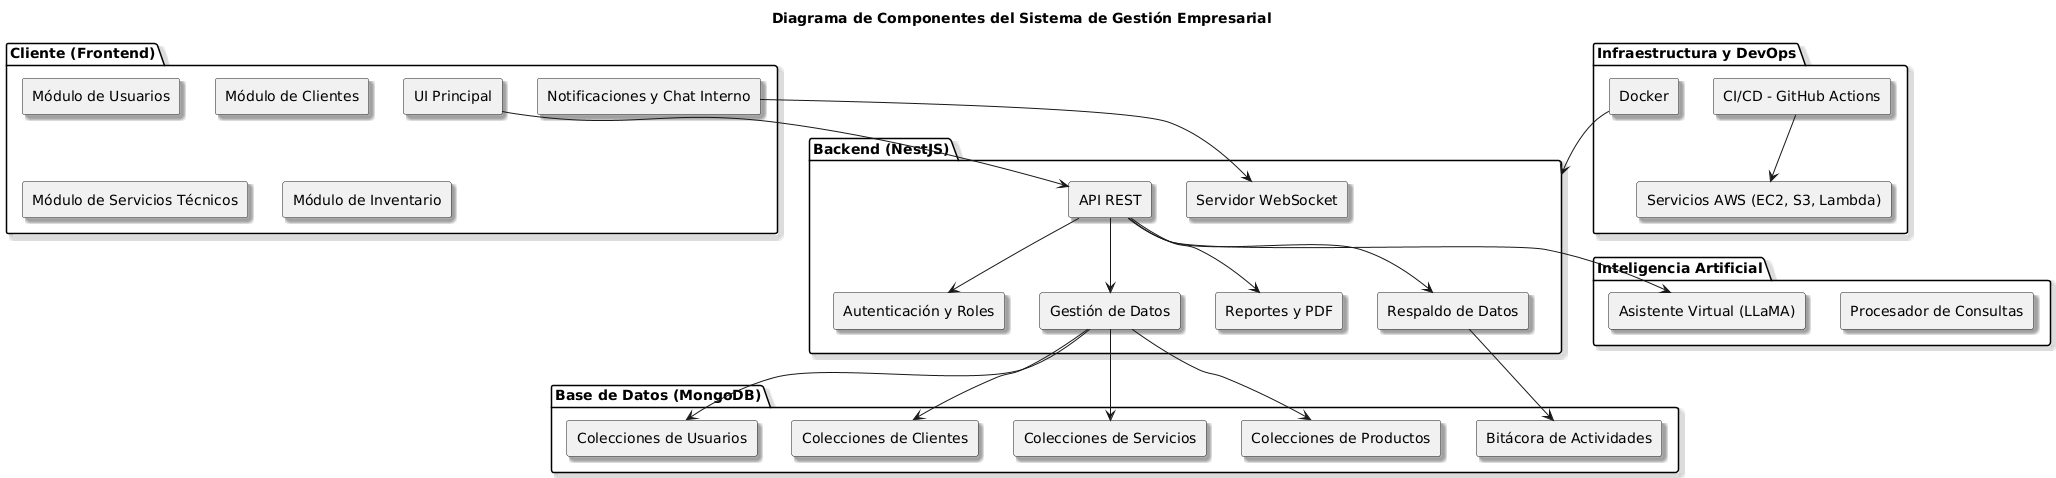
\includegraphics[width=0.6\textwidth]{componentes-sistema.png}
	\caption{Módulos principales del sistema de gestión y sus interacciones.}
	\label{fig:modulos}
\end{figure}

	
\section{Especificación técnica}

El sistema será accesible mediante una aplicación web dividida en backend y frontend independientes. Los módulos funcionales operan de forma integrada a través de APIs RESTful, alineados con los flujos reales de la empresa. La arquitectura es modular, escalable y mantenible.

\subsection*{Tecnologías utilizadas}

\begin{itemize}
	\item \textbf{Backend:} NestJS con TypeScript sobre Node.js. Arquitectura modular compuesta por controladores, servicios, repositorios, DTOs y validaciones centralizadas usando \texttt{class-validator}. Esta estructura permite separar responsabilidades y mantener el sistema escalable y mantenible.
	\item \textbf{Frontend:} React.js con TypeScript. Arquitectura basada en \textbf{Screaming Architecture} y \textbf{Clean Architecture}, lo cual permite que la estructura del proyecto refleje claramente sus funcionalidades, promoviendo una alta cohesión y bajo acoplamiento entre componentes.
	\item \textbf{Base de datos:} MongoDB, con soporte para múltiples empresas (multitenant) mediante aislamiento lógico de datos.
	\item \textbf{Interfaz de usuario:} HTML5 y CSS3, apoyado con Figma para diseño de prototipos y TalwindCSS para componentes accesibles y responsivos.
	\item \textbf{Comunicación:} WebSockets para mensajería interna en tiempo real y actualizaciones automáticas de estados.
	\item \textbf{Correo electrónico:} Protocolo SMTP para el envío automático de notificaciones operativas a usuarios internos y clientes.
	\item \textbf{Control de versiones e integración continua:} Git para versionamiento y GitHub Actions para automatización del pipeline CI/CD.
	\item \textbf{Contenerización y despliegue:} Uso de Docker para encapsular servicios, con despliegue en AWS (EC2 para la aplicación, S3 para archivos y Lambda para procesos automatizados).
\end{itemize}


\subsection*{Alcance funcional}

El proyecto contempla como mínimo la implementación de los siguientes módulos:

\begin{itemize}
	\item Gestión de empleados con autenticación y roles.
	\item Registro y administración de clientes individuales y empresariales.
	\item Flujo completo de servicios técnicos con seguimiento automatizado.
	\item Catálogo digital de productos e insumos.
	\item Notificaciones por correo y sistema de comunicación interna.
	\item Respaldo automático configurable y generación de reportes técnicos.
	\item Soporte multitenant para múltiples compañías, según la empresa seleccionada al iniciar sesión.
\end{itemize}

\subsection*{Criterios de finalización}

El sistema se considerará funcional cuando:

\begin{itemize}
	\item Cada módulo esté implementado y probado funcionalmente.
	\item Los casos de uso estén validados y documentados.
	\item El sistema esté desplegado en un entorno de pruebas funcional.
	\item Se incluya documentación técnica, manual de usuario y código fuente organizado.
	\item Se entregue una carpeta digital con el PDF final, código fuente comprimido y apéndices con el listado de código.
\end{itemize}


	
	Cada módulo será considerado finalizado cuando cumpla con los casos de uso definidos, haya sido probado funcionalmente y esté debidamente documentado. Además, el sistema deberá encontrarse desplegado en un entorno de pruebas funcional para su demostración.
	
	La Figura~\ref{fig:modulos} muestra un esquema general de los módulos definidos, y la Figura~\ref{fig:casosuso} representa los principales casos de uso considerados para la validación del sistema.
	
	\vspace{0.5cm}
	
	%Este texto SÍ debe incluirse para que la propuesta pueda ser aceptada.
	Al concluir el proyecto de integración se entregará a la Coordinación de Estudios de Ingeniería en Computación una carpeta digital que incluirá el reporte final del proyecto en un archivo PDF (sin restricciones)\footnote{Debe poder visualizarse sin solicitar contraseña}, el código fuente del proyecto en un archivo comprimido (sin restricciones)\footnote{Debe poder descomprimirse sin solicitar contraseña}. Además, la sección de apéndices del reporte final contendrá al menos un listado del código fuente desarrollado.


	\section{Calendario de actividades}

Las actividades a realizar durante el Trimestre 2025-Invierno en la UEA Proyecto de Integración de Ingeniería en Computación I (clave 1100113), con un valor de 18 créditos y una duración total de 198 horas, se presentan en la Tabla~\ref{table:calendarioActividades}.

\begin{longtable}{p{0.05\textwidth} p{0.4\textwidth} p{0.1\textwidth} p{0.35\textwidth}}
	\caption{Listado de actividades a realizar durante el Trimestre 2025-Invierno.}
  	\label{table:calendarioActividades}\\
	\toprule
	\textbf{No.} & \textbf{Actividad} & \textbf{Horas} & \textbf{Entregable} \\
	\hline
	\endfirsthead

	\multicolumn{4}{c}{\textbf{Continuación de la Tabla \ref{table:calendarioActividades}}}\\
	\hline
	\textbf{No.} & \textbf{Actividad} & \textbf{Horas} & \textbf{Entregable} \\
	\hline
	\endhead

	\hline
	\endlastfoot

	1 & Levantamiento de requerimientos y análisis del sistema actual en AironTools. & 20 & Documento de requerimientos \\
	\midrule

	2 & Diseño de arquitectura del sistema y definición de módulos. & 20 & Diagramas de arquitectura y diseño técnico \\
	\midrule

	3 & Desarrollo del módulo de autenticación y gestión de usuarios. & 25 & Módulo funcional con control de acceso y roles \\
	\midrule

	4 & Desarrollo del módulo de gestión de clientes. & 20 & Registro, historial y vista de clientes implementados \\
	\midrule

	5 & Desarrollo del módulo de servicios técnicos (flujo completo). & 25 & Módulo de flujo de servicio técnico automatizado \\
	\midrule

	6 & Desarrollo del módulo de inventario. & 20 & Registro, movimientos y alertas de inventario \\
	\midrule

	7 & Implementación de sistema de notificaciones y comunicación interna. & 20 & Notificaciones por correo, alertas internas y tareas asignadas \\
	\midrule

	8 & Pruebas funcionales e integración de los módulos. & 20 & Reporte de pruebas, casos de uso validados \\
	\midrule

	9 & Despliegue en entorno de pruebas y revisión técnica. & 15 & Sistema desplegado en servidor y documentación preliminar \\
	\midrule

	10 & Documentación técnica y elaboración de manual de usuario. & 13 & Manual de usuario, guía de instalación y documentación del sistema \\
	\bottomrule
\end{longtable}

\footnotetext{La planeación cubre el análisis, diseño, desarrollo, pruebas, despliegue y documentación del sistema, abarcando las 198 horas correspondientes a la UEA mencionada.}




\section{Factibilidad técnica y operativa}

\subsection{Factibilidad técnica}

El proyecto de desarrollo del sistema de gestión empresarial para AironTools es técnicamente viable, ya que el responsable del desarrollo cuenta con los conocimientos y habilidades necesarios para implementar los módulos definidos en el tiempo estipulado. Entre las competencias destacadas se encuentran:

\begin{itemize}
	\item Conocimientos avanzados en desarrollo web fullstack utilizando tecnologías como React.js, TypeScript y NestJS.
	\item Experiencia en diseño e implementación de arquitecturas modulares y sistemas empresariales.
	\item Habilidad en pruebas, documentación técnica y despliegue de sistemas.
\end{itemize}

Los recursos disponibles para el desarrollo y pruebas del sistema son los siguientes:

\begin{itemize}
	\item Equipos de cómputo con procesadores Intel Core i7, 16 GB de RAM y almacenamiento SSD.
	\item Acceso a entornos locales y servidores remotos para pruebas y despliegue del sistema.
	\item Conectividad de red estable para realizar pruebas multiusuario y simulaciones reales.
\end{itemize}

Las herramientas que se utilizarán durante el desarrollo incluyen:

\begin{itemize}
	\item \textbf{Frontend:} React.js con TypeScript, Figma para prototipado, y TalwindCSS para diseño de interfaz.
	\item \textbf{Backend:} NestJS con Node.js y MongoDB como base de datos.
	\item \textbf{Control de versiones:} Git y GitHub.
	\item \textbf{Contenedores y despliegue:} Docker, GitHub Actions para integración y entrega continua.
\end{itemize}

No se requieren recursos físicos adicionales ni licencias de software especiales, ya que todas las herramientas son de uso libre o ya están disponibles.

\subsection{Factibilidad operativa}

El sistema propuesto presenta una alta factibilidad operativa dentro de la empresa AironTools, por las siguientes razones:

\begin{itemize}
	\item \textbf{Adaptabilidad a los procesos actuales:} El sistema está alineado con los flujos de trabajo reales de la empresa, por lo que su adopción no requerirá una reestructuración significativa.
	
	\item \textbf{Aceptación organizacional:} El proyecto cuenta con el respaldo directo del jefe de área, el Ing. Víctor Benjamín Aguilar Orocio, responsable de la implementación en la empresa.
	
	\item \textbf{Capacitación del personal:} Se prevé una estrategia de introducción y formación progresiva, asegurando que los empleados comprendan y utilicen el sistema eficazmente.
	
	\item \textbf{Facilidad de uso y soporte:} La interfaz estará diseñada con criterios de usabilidad, y el sistema incluirá funciones de ayuda y comunicación interna que facilitarán su soporte continuo.
	
	\item \textbf{Extensibilidad y mantenimiento:} Gracias a su arquitectura modular, el sistema podrá adaptarse a futuras necesidades o integrarse con nuevas tecnologías sin comprometer su estabilidad.
\end{itemize}

\vspace{0.5cm}
\section{Estimación de costos}

La presente sección muestra una estimación comercial del capital necesario para el desarrollo del sistema de gestión empresarial propuesto, considerando tanto los recursos técnicos como el valor del trabajo intelectual involucrado. Se han incluido costos asociados a infraestructura, herramientas, servicios y personal. Esta estimación representa una aproximación realista en caso de que el proyecto se desee escalar o comercializar.

La estimación de costos del proyecto se presenta en la Tabla~\ref{table:tablaCostos}.

\begin{longtable}{m{6.5cm} m{4.5cm} m{4cm}}
	\caption{Estimación de costos del proyecto.}
  	\label{table:tablaCostos}\\
  	\toprule
	\textbf{Descripción} & \textbf{Costo unitario (MXN)} & \textbf{Costo total (MXN)} \\
	\hline
	\endfirsthead

	\multicolumn{3}{c}{\textbf{Continuación de la Tabla \ref{table:tablaCostos}}}\\
	\hline
	\textbf{Descripción} & \textbf{Costo unitario (MXN)} & \textbf{Costo total (MXN)} \\
	\hline
	\endhead

	\hline
	\endlastfoot

Trabajo de desarrollo (fullstack, 8 meses) & \$9,974.00 $\times$ 8 meses & \$79,792.00 \\
\midrule

Desarrollo frontend de apoyo (8 meses) & \$8,500.00 $\times$ 8 meses & \$68,000.00 \\
\midrule

Computadora personal del desarrollador principal & — & \$12,000.00 \\
\midrule

Computadora personal de la desarrolladora frontend & — & \$12,000.00 \\
\midrule

Servidor local Linux & — & \$8,000.00 \\
\midrule

Cámara digital para registro de productos & — & \$800.00 \\
\midrule

Servicios en la nube (Amazon Web Services, total 6 meses) & \$92.29 USD $\approx$ \$1,841.19 & \$1,841.19 \\
\midrule

Gestión de repositorios (GitHub Teams, plan anual) & \$96.00 USD $\approx$ \$1,915.20 & \$1,915.20 \\
\midrule

\textbf{Costo total estimado} & — & \textbf{\$184,348.39} \\
\bottomrule
\end{longtable}

\noindent
\textbf{Nota:} Los montos fueron calculados con base en recibos de nómina, facturas y registros reales generados durante el desarrollo del sistema. Estos datos provienen de pagos y compras efectuados por la empresa, tanto al responsable del proyecto como al personal de apoyo. Los precios de herramientas, servicios y equipos se estimaron conforme a comprobantes de adquisición y consumo. En caso de ser necesario, la empresa puede proporcionar la documentación correspondiente bajo solicitud formal.
